\documentclass[11pt]{amsart}
\usepackage[a4paper,margin=1in]{geometry}
\usepackage{amssymb}
\usepackage{tikz}
\usepackage[font=small,labelfont=bf]{caption}
\usepackage[hidelinks]{hyperref}

\colorlet{copper}{orange!75!black}
\colorlet{inkmuted}{black!60}
\tikzset{thin/.style={line width=0.4pt}}

\newtheorem{theorem}{Theorem}
\theoremstyle{remark}
\newtheorem{remark}[theorem]{Remark}

\title{Every Other Residue}
\author{Vamshi Jandhyala}
\address{London, United Kingdom}
\email{vamshi.jandhyala@gmail.com}

\begin{document}

\begin{abstract}
Let $A$ and $B$ be sets of $2^k$ residues modulo $2^{k+1}$, each reducing modulo $2^k$ to every residue exactly once. We show that $A$ and $B$ can be matched so that the $2^k$ sums are pairwise distinct modulo $2^{k+1}$, answering a question on Mathematics Stack Exchange. More precisely, the sums can be made exactly the even residues or exactly the odd residues, according to the parity of the number of elements of $A$ and $B$ in the upper half, and never the other class. This is a case of Snevily's conjecture for cyclic groups of even order, which remains open in general. The proof is a short induction that halves both sets, and it is formally verified in Lean.
\end{abstract}

\maketitle

\section{The question}

Take two sets $A$, $B$ of $n$ residues modulo $m$. Can they be matched in pairs so that the $n$ sums are pairwise distinct? For odd $m$ the answer is always yes: Snevily conjectured this in 1999~\cite{Snevily}, Dasgupta, Károlyi, Serra and Szegedy proved it for cyclic groups~\cite{DKSS}, and Arsovski for all abelian groups of odd order~\cite{Arsovski}. For even $m$ it can fail. The even residues modulo $4$, matched with themselves, give sums $0+0,2+2$ or $0+2,2+0$, and either way the two sums agree. Snevily conjectured that this is essentially the only obstruction: in $\mathbb Z/m$ with $m$ even, a matching with distinct sums exists unless $A$ and $B$ are translates of the same cyclic subgroup of even order~\cite{Snevily,DKSS}. That conjecture is open.

In December 2016 a user of Mathematics Stack Exchange asked about one case~\cite{MSE}. Let $A$ and $B$ be sets of $2^k$ residues modulo $2^{k+1}$, each of which reduces modulo $2^k$ to every residue exactly once. Can they always be matched with distinct sums modulo $2^{k+1}$? Such sets are never translates of the subgroup of even residues, since a translate of that subgroup reduces modulo $2^k$ to only half the residues, so the question is a case of the even-order conjecture. Before reading on, try $k=1$: $A$ and $B$ each contain one of $0,2$ and one of $1,3$.

Write each element of $A$ as $a=r+2^ke_r$ with $0\le r<2^k$ and $e_r\in\{0,1\}$; so $r$ is its residue modulo $2^k$, and $e_r=1$ when $a$ lies in the upper half $[2^k,2^{k+1})$. Write $B$ the same way with bits $f_r$, and put
\[
p=\Bigl(\sum_re_r+\sum_rf_r\Bigr)\bmod 2,
\]
the parity of the number of upper-half elements of $A$ and $B$ together.

\begin{theorem}\label{thm:main}
For every $k\ge0$ there is a matching of $A$ with $B$ whose $2^k$ sums are exactly the residues modulo $2^{k+1}$ of parity $p$. No matching has pairwise distinct sums of parity $1-p$.
\end{theorem}

For $k=1$ with $A=\{0,3\}$ and $B=\{2,1\}$ (so $e=(0,1)$, $f=(1,0)$ and $p=0$), matching $0$ with $2$ and $3$ with $1$ gives the even sums $2$ and $0$; the other matching gives $1$ and $1$.

\section{Why the top bit has to work}

A matching pairs the residue $r$ of $A$ with the residue $\pi(r)$ of $B$, for a permutation $\pi$ of $\mathbb Z/2^k$. The sums can never be distinct modulo $2^k$: the $r+\pi(r)$ add up to twice $0+1+\dots+(2^k-1)$, which is $0$ modulo $2^k$, while the $2^k$ residues add up to $2^{k-1}(2^k-1)$, which is not, for $k\ge1$. So some sums always agree modulo $2^k$, and a good matching is one in which every two sums that agree modulo $2^k$ fall in opposite halves. The bits $e_r$ and $f_r$ decide the halves, and the proof arranges them.

The second statement of Theorem~\ref{thm:main} is the same kind of count one level up. The residues $r$ of $A$ add up to $0+1+\dots+(2^k-1)$, and so do those of $B$, so every matching has total $2^k(2^k-1)+2^k\sum_r(e_r+f_r)$. If its sums are pairwise distinct of parity $q$, they are all the residues $2s+q$ with $s<2^k$, whose total is $2^k(2^k-1)+2^kq$. Comparing the two totals modulo $2^{k+1}$ gives $2^k\sum_r(e_r+f_r)\equiv2^kq$, that is, $q\equiv p\pmod 2$.

\section{Halving}

Split both sets by their last bit and halve. If $A$ reduces to every residue modulo $2^k$ once, its even elements reduce to the even residues once each, so halving them gives $2^{k-1}$ residues modulo $2^k$ that reduce to every residue modulo $2^{k-1}$ once. The odd elements, after subtracting $1$ and halving, do the same. Halving keeps the upper-half bit, since $a\ge2^k$ exactly when $\lfloor a/2\rfloor\ge2^{k-1}$. So each half is a smaller instance of the same problem.

\begin{proof}[Proof of Theorem~\ref{thm:main}, first statement]
Induction on $k$. For $k=0$ the sets are single residues modulo $2$, and the one sum has parity $e_0+f_0=p$.

For $k\ge1$ split $A=A_0\cup A_1$ and $B=B_0\cup B_1$ into even and odd elements, and let
\[
X_0=A_0/2,\quad X_1=(A_1-1)/2,\quad Y_0=B_0/2,\quad Y_1=(B_1-1)/2,
\]
four instances of size $2^{k-1}$ in $\mathbb Z/2^k$. Writing $p(X,Y)$ for the parity count of a pair,
\[
p(X_0,Y_0)+p(X_1,Y_1)\equiv p(X_0,Y_1)+p(X_1,Y_0)\equiv p\pmod2,
\]
because each side counts every upper-half element of $A$ and $B$ once. Matching $x\in X_c$ with $y\in Y_d$ means matching $2x+c$ with $2y+d$, with sum $2(x+y)+c+d$.

\emph{Case $p=0$.} Match $A_0$ with $B_0$ and $A_1$ with $B_1$. The two counts $p(X_0,Y_0)$ and $p(X_1,Y_1)$ add to $0$, so they are equal, say to $q$. By induction the sums $x+y$ in each half run over the residues of parity $q$ modulo $2^k$. In $\mathbb Z/2^{k+1}$ the sums are then $2t$ and $2t+2=2(t+1)$ for every $t$ of parity $q$; as $t+1$ has parity $1-q$, together these are all the even residues.

\emph{Case $p=1$.} Match $A_0$ with $B_1$ and $A_1$ with $B_0$. The sums are $2t+1$ for $t$ of parity $p(X_0,Y_1)$, and $2t+1$ for $t$ of parity $p(X_1,Y_0)$. These two parities add to $1$, so they differ, and the sums are all the odd residues.
\end{proof}

The proof is also an algorithm: split by the last bit, choose the case by one parity count, recurse, in time proportional to $k\,2^k$. Figure~\ref{fig:halving} traces its first step on an example with $k=3$, and Table~\ref{tab:ex} gives the final matching.

\begin{figure}[ht]
\centering
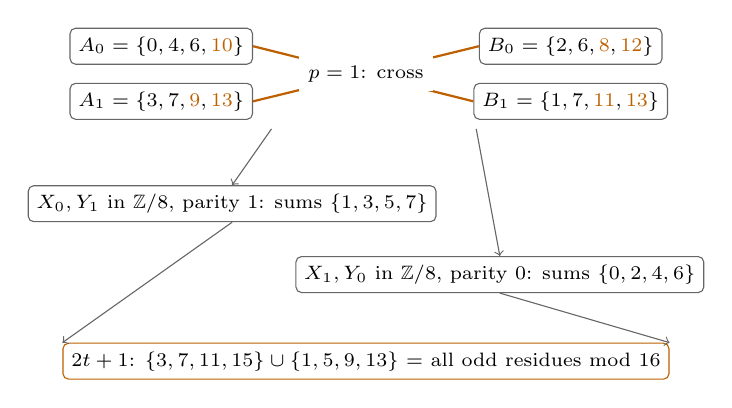
\begin{tikzpicture}
  \tikzset{bx/.style={draw=inkmuted, rounded corners=2pt, inner sep=3pt, font=\scriptsize}}
\node[bx] (a0) at (0,0) {$A_0=\{0,4,6,\textcolor{copper}{10}\}$};
\node[bx] (a1) at (0,-0.7) {$A_1=\{3,7,\textcolor{copper}{9},\textcolor{copper}{13}\}$};
\node[bx] (b0) at (5.2,0) {$B_0=\{2,6,\textcolor{copper}{8},\textcolor{copper}{12}\}$};
\node[bx] (b1) at (5.2,-0.7) {$B_1=\{1,7,\textcolor{copper}{11},\textcolor{copper}{13}\}$};
\draw[copper, thick] (a0.east) -- (b1.west); \draw[copper, thick] (a1.east) -- (b0.west);
\node[font=\scriptsize, fill=white] at (2.6,-0.35) {$p=1$: cross};
\node[bx] (h1) at (0.9,-2.0) {$X_0,Y_1$ in $\mathbb Z/8$, parity $1$: sums $\{1,3,5,7\}$};
\node[bx] (h2) at (4.3,-2.9) {$X_1,Y_0$ in $\mathbb Z/8$, parity $0$: sums $\{0,2,4,6\}$};
\draw[->, inkmuted] (1.4,-1.05) -- (h1.north); \draw[->, inkmuted] (4.0,-1.05) -- (h2.north);
\node[bx, draw=copper] (fin) at (2.6,-4.0) {$2t+1$: $\{3,7,11,15\}\cup\{1,5,9,13\}$ = all odd residues mod $16$};
\draw[->, inkmuted] (h1.south) -- (fin.north west); \draw[->, inkmuted] (h2.south) -- (fin.north east);

\end{tikzpicture}
\caption{The first step of the proof on $A=\{0,9,10,3,4,13,6,7\}$ and $B=\{8,1,2,11,12,13,6,7\}$ modulo $16$. Upper-half elements are in copper: three in $A$ and four in $B$, so $p=1$ and evens are matched with odds. Halving gives two instances in $\mathbb Z/8$ with parities $1$ and $0$; their sums are the odd and the even residues modulo $8$, and $t\mapsto2t+1$ turns them into complementary halves of the odd residues modulo $16$.}
\label{fig:halving}
\end{figure}

\begin{table}[ht]
\centering
\begin{tabular}{l|rrrrrrrr}
\hline
$A$ & $0$ & $4$ & $10$ & $6$ & $9$ & $13$ & $3$ & $7$\\
$B$ & $7$ & $11$ & $1$ & $13$ & $8$ & $12$ & $2$ & $6$\\
\hline
sum mod $16$ & $7$ & $15$ & $11$ & $3$ & $1$ & $9$ & $5$ & $13$\\
\hline
\end{tabular}
\caption{The matching the proof produces for the sets of Figure~\ref{fig:halving}: its sums are the eight odd residues modulo $16$.}
\label{tab:ex}
\end{table}

\begin{remark}
The theorem does not follow from the odd-order results, and the halving does not obviously extend to the full even-order conjecture: halving needs both sets to split evenly by their last bit at every level, which is exactly what the hypothesis on residues modulo $2^k$ provides.
\end{remark}

\section{Verification}

Both statements of Theorem~\ref{thm:main}, and the fact in Section~2 that the sums are never distinct modulo $2^k$, are proved in Lean~4 with Mathlib~\cite{mathlib}, by the arguments above; sets are encoded by their bit vectors $e$, $f$ and a matching by a permutation of $\{0,\dots,2^k-1\}$. A Python script checks the theorem by exhaustive search for $k\le3$ (and the impossibility of the other parity for $k\le2$), runs the recursive construction on $3000$ random instances for each $k\le12$, and catches two planted errors (the two cases swapped, and a parity count that ignores $B$). A C program searches all pairs for $k\le3$ independently. Code and Lean files are at~\cite{repo}.

\section*{Acknowledgments}

The question is due to the Mathematics Stack Exchange user now shown as user160886. The analysis, the computations and the Lean formalisation were carried out with Claude Opus~5.5 (Anthropic). The author is responsible for the content.

\begin{thebibliography}{9}
\bibitem{Arsovski} B.~Arsovski, \emph{A proof of Snevily's conjecture}, Israel J. Math. 182 (2011), 505--508.
\bibitem{DKSS} S.~Dasgupta, G.~Károlyi, O.~Serra and B.~Szegedy, \emph{Transversals of additive Latin squares}, Israel J. Math. 126 (2001), 17--28.
\bibitem{MSE} user160886, \emph{A Combinatorial problem involving $\mathbf{Z}/2^k\mathbf{Z}$}, Mathematics Stack Exchange question 2060312 (2016), \url{https://math.stackexchange.com/q/2060312}.
\bibitem{Snevily} H.~S.~Snevily, \emph{The Cayley addition table of $\mathbb Z_n$}, Amer. Math. Monthly 106 (1999), 584--585.
\bibitem{mathlib} The mathlib Community, \emph{The Lean mathematical library}, in: Proc. 9th ACM SIGPLAN Int. Conf. on Certified Programs and Proofs (CPP 2020), 367--381.
\bibitem{repo} V.~Jandhyala, code and Lean proofs, \url{https://github.com/jvvk/mathematics/tree/main/every-other-residue}.
\end{thebibliography}

\end{document}
